\begin{block}{At a Glance}
  Beginning in Nov. 2015, repeated intense rainfall events associated with mesoscale convective activity caused severe flooding along the Paraguay-Paran\'{a} river system (\cref{fig:study-area}, red box), \emph{displacing over 170000 people}.
  We use a weather typing approach within a diagnostic framework to show that:
  \begin{itemize}
    \item Moisture and energy advection via the South American Low-Level Jet \cite[SALLJ;][]{Marengo:2012cm}, particularly during ``No-Chaco'' events \cite{Vera:2006ib} favored mesoscale convective activity
    \item Strong El Ni\~{n}o and active MJO favored a strong SALLJ but an Atlantic dipole pattern influenced the jet's exit region
    \item Numerical forecasts predicted enhanced risk of heavy rainfall at the seasonal scale, but biases in spatial patterns suggest difficulties representing Pacific-Atlantic interaction
    \item Uncorrected sub-seasonal model forecasts of rainfall had limited skill beyond 10-15 days; use of Model Output Statistics -- particularly methods that correct both spatial patterns and magnitudes -- substantially improved forecast skill
  \end{itemize}
  \begin{mdframed}
  \begin{figure}
  	\noindent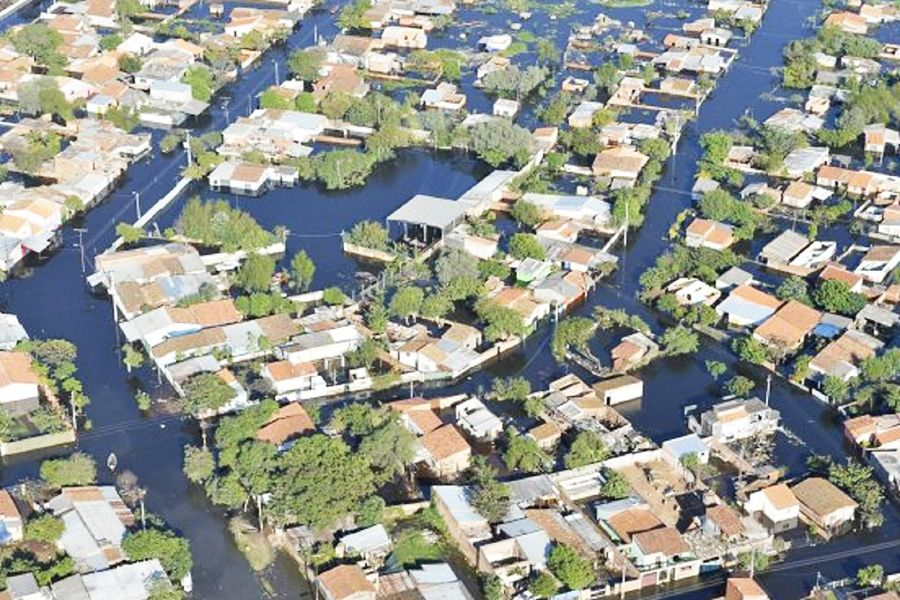
\includegraphics[width=0.45\textwidth]{asuncion-inundaciones.jpg}~
    \noindent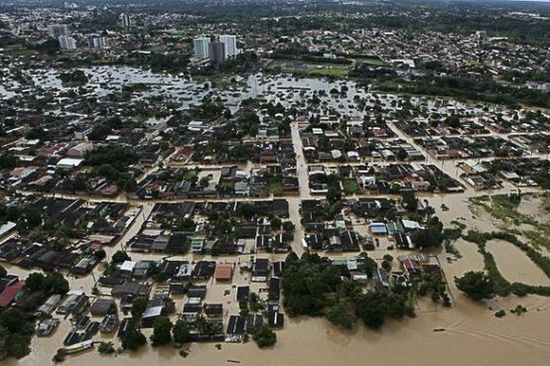
\includegraphics[width=0.45\textwidth]{rio-py-banados.jpg}
  	\caption{
  		Asuncion, Paraguay, 2015-16
  	}
    \label{fig:floods}
  \end{figure}
  \end{mdframed}
\end{block}
